\begin{figure}[h]
    \centering
    \begin{subfigure}[b]{0.32\textwidth}
        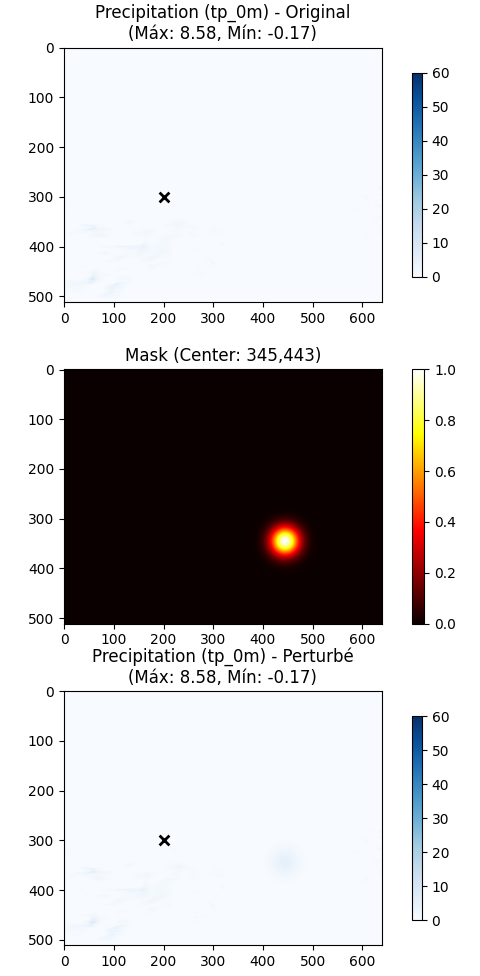
\includegraphics[width=\textwidth]{Images/titan_rain_perturbations/perturbed_c_tp_0m.png}
        \caption{Channel aro\_tp\_0m}
        \label{fig:titan_perturbed_aro_tp}
    \end{subfigure}
    \hfill
    \begin{subfigure}[b]{0.32\textwidth}
        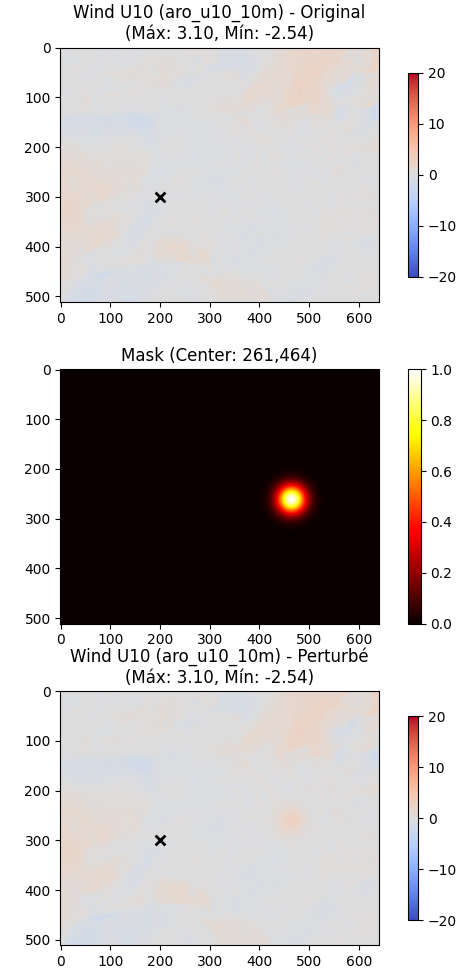
\includegraphics[width=\textwidth]{Images/titan_rain_perturbations/perturbed_c_u10_10m.png}
        \caption{Channel aro\_u10\_10m}
        \label{fig:titan_perturbed_aro_u10}
    \end{subfigure}
    \hfill
    \begin{subfigure}[b]{0.32\textwidth}
        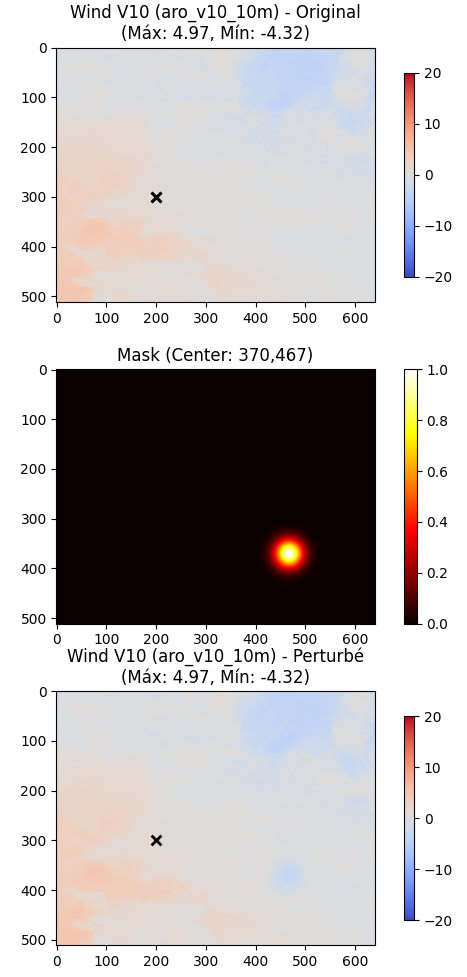
\includegraphics[width=\textwidth]{Images/titan_rain_perturbations/perturbed_c_v10_10m.png}
        \caption{Channel aro\_v10\_10m}
        \label{fig:titan_perturbed_aro_v10}
    \end{subfigure}
    \caption{Example of counterfactuals of Titan image channels from 18/11/2023}
    \label{fig:titan-rain-perturbations}
\end{figure}